\documentclass{article}

\usepackage[english]{babel}
\usepackage[letterpaper,top=2cm,bottom=2cm,left=3cm,right=3cm,marginparwidth=1.75cm]{geometry}
\usepackage{amsmath}
\usepackage{graphicx}
\usepackage{xcolor}
\usepackage[colorlinks=true, allcolors=blue]{hyperref}
\usepackage{placeins}
\usepackage{subcaption}
\usepackage{listings}

\lstset{
    language=Python,
    basicstyle=\ttfamily\footnotesize,
    keywordstyle=\color{blue!80!black}\bfseries,
    commentstyle=\color{green!60!black}\itshape,
    stringstyle=\color{orange!90!black},
    identifierstyle=\color{black},
    emphstyle=\color{purple!80!black}\bfseries,
    numbers=left,
    numberstyle=\tiny\color{gray!60},
    stepnumber=1,
    numbersep=10pt,
    tabsize=4,
    breaklines=true,
    breakatwhitespace=true,
    frame=none,
    backgroundcolor=\color{gray!8},
    showstringspaces=false,
    captionpos=b,
    xleftmargin=15pt,
    xrightmargin=5pt,
    aboveskip=12pt,
    belowskip=12pt,
    lineskip=0.8pt,
    moredelim=[s][\color{orange!90!black}]{'''}{'''},
    moredelim=[s][\color{orange!90!black}]{"""}{"""},
    literate={0}{{{\color{purple!80!black}0}}}1
             {1}{{{\color{purple!80!black}1}}}1
             {2}{{{\color{purple!80!black}2}}}1
             {3}{{{\color{purple!80!black}3}}}1
             {4}{{{\color{purple!80!black}4}}}1
             {5}{{{\color{purple!80!black}5}}}1
             {6}{{{\color{purple!80!black}6}}}1
             {7}{{{\color{purple!80!black}7}}}1
             {8}{{{\color{purple!80!black}8}}}1
             {9}{{{\color{purple!80!black}9}}}1
}
\graphicspath{{Images/}}

\title{PUNCH!}
\author{Kim Hyeong-Seok}

\begin{document}
\maketitle

\begin{abstract}
    PUNCH! is a mobile application designed to facilitate combat-style exercise using only a smartphone, enabling users to engage in physical activity even in confined spaces. This paper details the development and testing of PUNCH!, focusing on the utilization of smartphone sensors to track movement and classify punch types. The application employs advanced techniques such as orientation estimation, noise reduction, and deep learning models to achieve accurate motion detection and classification. The results demonstrate the feasibility of using smartphones for effective combat-style exercise, addressing common barriers to physical activity in modern lifestyles.
\end{abstract}

\section{Introduction}

Modern individuals often struggle to maintain a healthy lifestyle due to a lack of physical activity, chronic stress, and the demands of a busy daily routine. In particular, time and space constraints, financial burdens, and psychological barriers associated with exercise contribute to the growing difficulty of engaging in regular physical activity. To address these challenges, we developed PUNCH!, a mobile application that enables users to easily engage in combat-style exercise using only a smartphone, even within confined spaces.

The development and testing of this application were conducted using a MacBook Pro (M1, 2021) and an iPhone 14 Pro, which will hereafter be referred to as the smartphone. All data collection and code execution were performed exclusively on these two devices, and the application has not been tested on platforms other than iOS.

\section{Methods}

\subsection{Utilization of Smartphone Sensors}

\subsubsection{Measurement of Acceleration via Calibration and Differencing}

To isolate acceleration caused solely by device movement, a calibration process was performed by maintaining the smartphone in a standard orientation—perpendicular to the ground with the screen facing the user—for one second. The accelerometer readings obtained during this calibration were used as a reference, and subsequent acceleration measurements were compared against this baseline to estimate changes due exclusively to motion. This approach assumes gravitational acceleration as a constant bias, allowing for a simplified implementation that focuses on relative changes in acceleration.

However, gravitational force continuously affects accelerometer readings, and variations in device tilt or orientation can significantly alter the measured values. As such, ignoring the influence of gravity imposes a limitation on the accuracy of this method. The approach lacks the precision necessary to isolate pure translational acceleration. Consequently, we decided to incorporate a mathematically and physically grounded method for tracking the device’s orientation to account for gravitational effects more accurately.

\FloatBarrier
\begin{figure}
    \centering
    \includegraphics[width=\textwidth]{Images/data_difference_and_integration.png}
    \caption{Charts comparing raw data and differentiated data}
    \label{fig:data_difference_and_integration}
    \centering
    \includegraphics[width=\textwidth]{Images/error_3d_path.png}
    \caption{An image of 3-dimension path estimated with differentiated data}
    \label{fig:error_3d_path}
\end{figure}

\FloatBarrier
\subsubsection{Orientation Estimation Using the Accelerometer}

\FloatBarrier
\begin{figure}[h]
    \centering
    \includegraphics[width=7.5cm]{Images/accelerometer.png}
    \caption{Smartphone accelerometer axis orientation}
    \label{fig:accelerometer}
\end{figure}

The coordinate system of the smartphone's accelerometer follows the right-hand rule, as illustrated in Figure~\ref{fig:accelerometer}. The output values of the sensor are normalized by the gravitational acceleration $9.8\,\mathrm{m/s^2}$, and thus each axis returns a value in units of $g$.

When the smartphone is held vertically, such that the $xz$-plane is parallel to the ground and the screen is facing the user, the expected accelerometer reading due to gravity is:

\[
\begin{bmatrix}
0\\
-1\\
0
\end{bmatrix}
\]

Let $\begin{bmatrix}x&y&z\end{bmatrix}^\top$ be the first accelerometer reading obtained after calibration. By comparing this measurement to the reference vector, we can estimate the initial orientation of the device. Before doing so, the accelerometer vector must be normalized to ensure consistency in magnitude.

The orientation is estimated using a sequence of rotation matrices about the $x$-, $y$-, and $z$-axes:

\[
R_x(\theta_x) =
\begin{bmatrix}
1 & 0 & 0 \\
0 & \cos\theta_x & -\sin\theta_x \\
0 & \sin\theta_x & \cos\theta_x
\end{bmatrix}\]
\[R_y(\theta_y) =
\begin{bmatrix}
\cos\theta_y & 0 & \sin\theta_y \\
0 & 1 & 0 \\
-\sin\theta_y & 0 & \cos\theta_y
\end{bmatrix}\]
\[R_z(\theta_z) =
\begin{bmatrix}
\cos\theta_z & -\sin\theta_z & 0 \\
\sin\theta_z & \cos\theta_z & 0 \\
0 & 0 & 1
\end{bmatrix}
\]

Assuming that the orientation angles $\theta_x$, $\theta_y$, and $\theta_z$ represent rotations about the respective axes, the rotated reference vector becomes:

\[
\begin{bmatrix}
x\\
y\\
z
\end{bmatrix}
=
R_y(\theta_y) \cdot R_x(\theta_x) \cdot R_z(\theta_z) \cdot
\begin{bmatrix}
0\\
-1\\
0
\end{bmatrix}
=
R_y(\theta_y) \cdot R_x(\theta_x) \cdot
\begin{bmatrix}
\sin\theta_z\\
-\cos\theta_z\\
0
\end{bmatrix}
=
R_y(\theta_y) \cdot
\begin{bmatrix}
\sin\theta_z\\
-\cos\theta_x \cos\theta_z\\
-\sin\theta_x \cos\theta_z
\end{bmatrix}
\]

Multiplying out the rotations yields:

\[
\begin{bmatrix}
x\\
y\\
z
\end{bmatrix}
=
\begin{bmatrix}
\cos\theta_y \sin\theta_z - \sin\theta_x \sin\theta_y \cos\theta_z \\
-\cos\theta_x \cos\theta_z \\
-\sin\theta_y \sin\theta_z - \sin\theta_x \cos\theta_y \cos\theta_z
\end{bmatrix}
\]

Since the accelerometer cannot determine rotation about the $y$-axis (yaw), we assume $\theta_y = 0$, simplifying the expression to:

\[
\begin{bmatrix}
x\\
y\\
z
\end{bmatrix}
=
\begin{bmatrix}
\sin\theta_z \\
-\cos\theta_x \cos\theta_z \\
\sin\theta_x \cos\theta_z
\end{bmatrix}
\]

From this simplified form, we can compute the orientation angles as follows. The $x$-component yields:

\[
\theta_z = \arcsin(x)
\]

To isolate $\theta_x$, we divide the third component by the second:

\[
\frac{z}{y} = \frac{\sin\theta_x \cos\theta_z}{-\cos\theta_x \cos\theta_z} = -\tan\theta_x \quad \Rightarrow \quad \theta_x = -\arctan\left(\frac{z}{y}\right)
\]

Let the initial orientation of the device be denoted by $\begin{bmatrix} \psi_0 & \theta_0 & \phi_0 \end{bmatrix}^\top$, corresponding to rotations around the $x$-, $y$-, and $z$-axes, respectively. Using the above method, we can estimate the initial orientation as:

\[
\begin{bmatrix}
\psi_0 \\
\theta_0 \\
\phi_0
\end{bmatrix}
=
\begin{bmatrix}
-\arctan\left(\frac{z}{y}\right) \\
0 \\
\arcsin(x)
\end{bmatrix}
\]

This method allows for a simple and effective estimation of the device’s initial pitch and roll, based on gravitational acceleration and assuming no initial yaw rotation.

\subsubsection{Valid Range for Accelerometer-Based Orientation Estimation}

When the smartphone is tilted around the $z$-axis, the $x$-axis acceleration value increases, while the $y$ and $z$ acceleration values approach zero. In this case, the term $z \div y$ in the previous orientation estimation formula diverges, leading to instability in the computation of $\theta_x$.

To address this issue, an alternative derivation using a product of the $y$ and $z$ components is proposed. Starting from the simplified rotation matrix:

\[
x = \sin\theta_z
\]
\[
y \cdot z = -\cos\theta_x \cos\theta_z \cdot \sin\theta_x \cos\theta_z 
= -\sin\theta_x \cos\theta_x \cdot \cos^2\theta_z 
= -\sin\theta_x \cos\theta_x \cdot (1 - \sin^2\theta_z)
= \frac{1}{2} \sin(2\theta_x) \cdot (x^2 - 1)
\]

From this, we can isolate $\theta_x$ as:

\[
\theta_x = \frac{1}{2} \arcsin\left(\frac{y \cdot z}{x^2 - 1}\right)
\]

However, this formulation also fails when the $x$-axis acceleration value approaches $1$ or $-1$, i.e., when $\theta_z \rightarrow \pm \frac{\pi}{2}$, which corresponds to tilting the smartphone to 90 degrees around the $z$-axis. In this situation, the denominator $x^2 - 1$ approaches zero, causing the expression to diverge and leading to instability in the calculation of $\theta_x$.

Empirical tests showed that when the tilt angle exceeds approximately $80^\circ$, the accelerometer data becomes increasingly noisy and unreliable, as illustrated in Figure~\ref{fig:valid_range_test}. In such cases, the estimated $\theta_x$ value becomes extremely large and physically implausible.

To ensure reliable orientation estimation, we restrict the accelerometer-based calculation of orientation (Section~2.1.2) to cases where the cosine similarity between the reference vector $\mathbf{g}_{ref} = \begin{bmatrix} 0 & -1 & 0 \end{bmatrix}^\top$ and the normalized acceleration vector $\mathbf{a}$ is greater than $0.5$, which corresponds to a maximum tilt angle of approximately $60^\circ$ from the ideal upright orientation:

\[
\cos\theta = \frac{\mathbf{g}_{ref} \cdot \mathbf{a}}{\|\mathbf{g}_{ref}\| \|\mathbf{a}\|} = \frac{-a_y}{\|\mathbf{a}\|} > 0.5
\]

If the initial orientation does not satisfy this condition, the user is prompted to hold the device in an upright position to proceed with calibration.

\FloatBarrier
\begin{figure}[h]
    \begin{subfigure}{0.5\textwidth}
        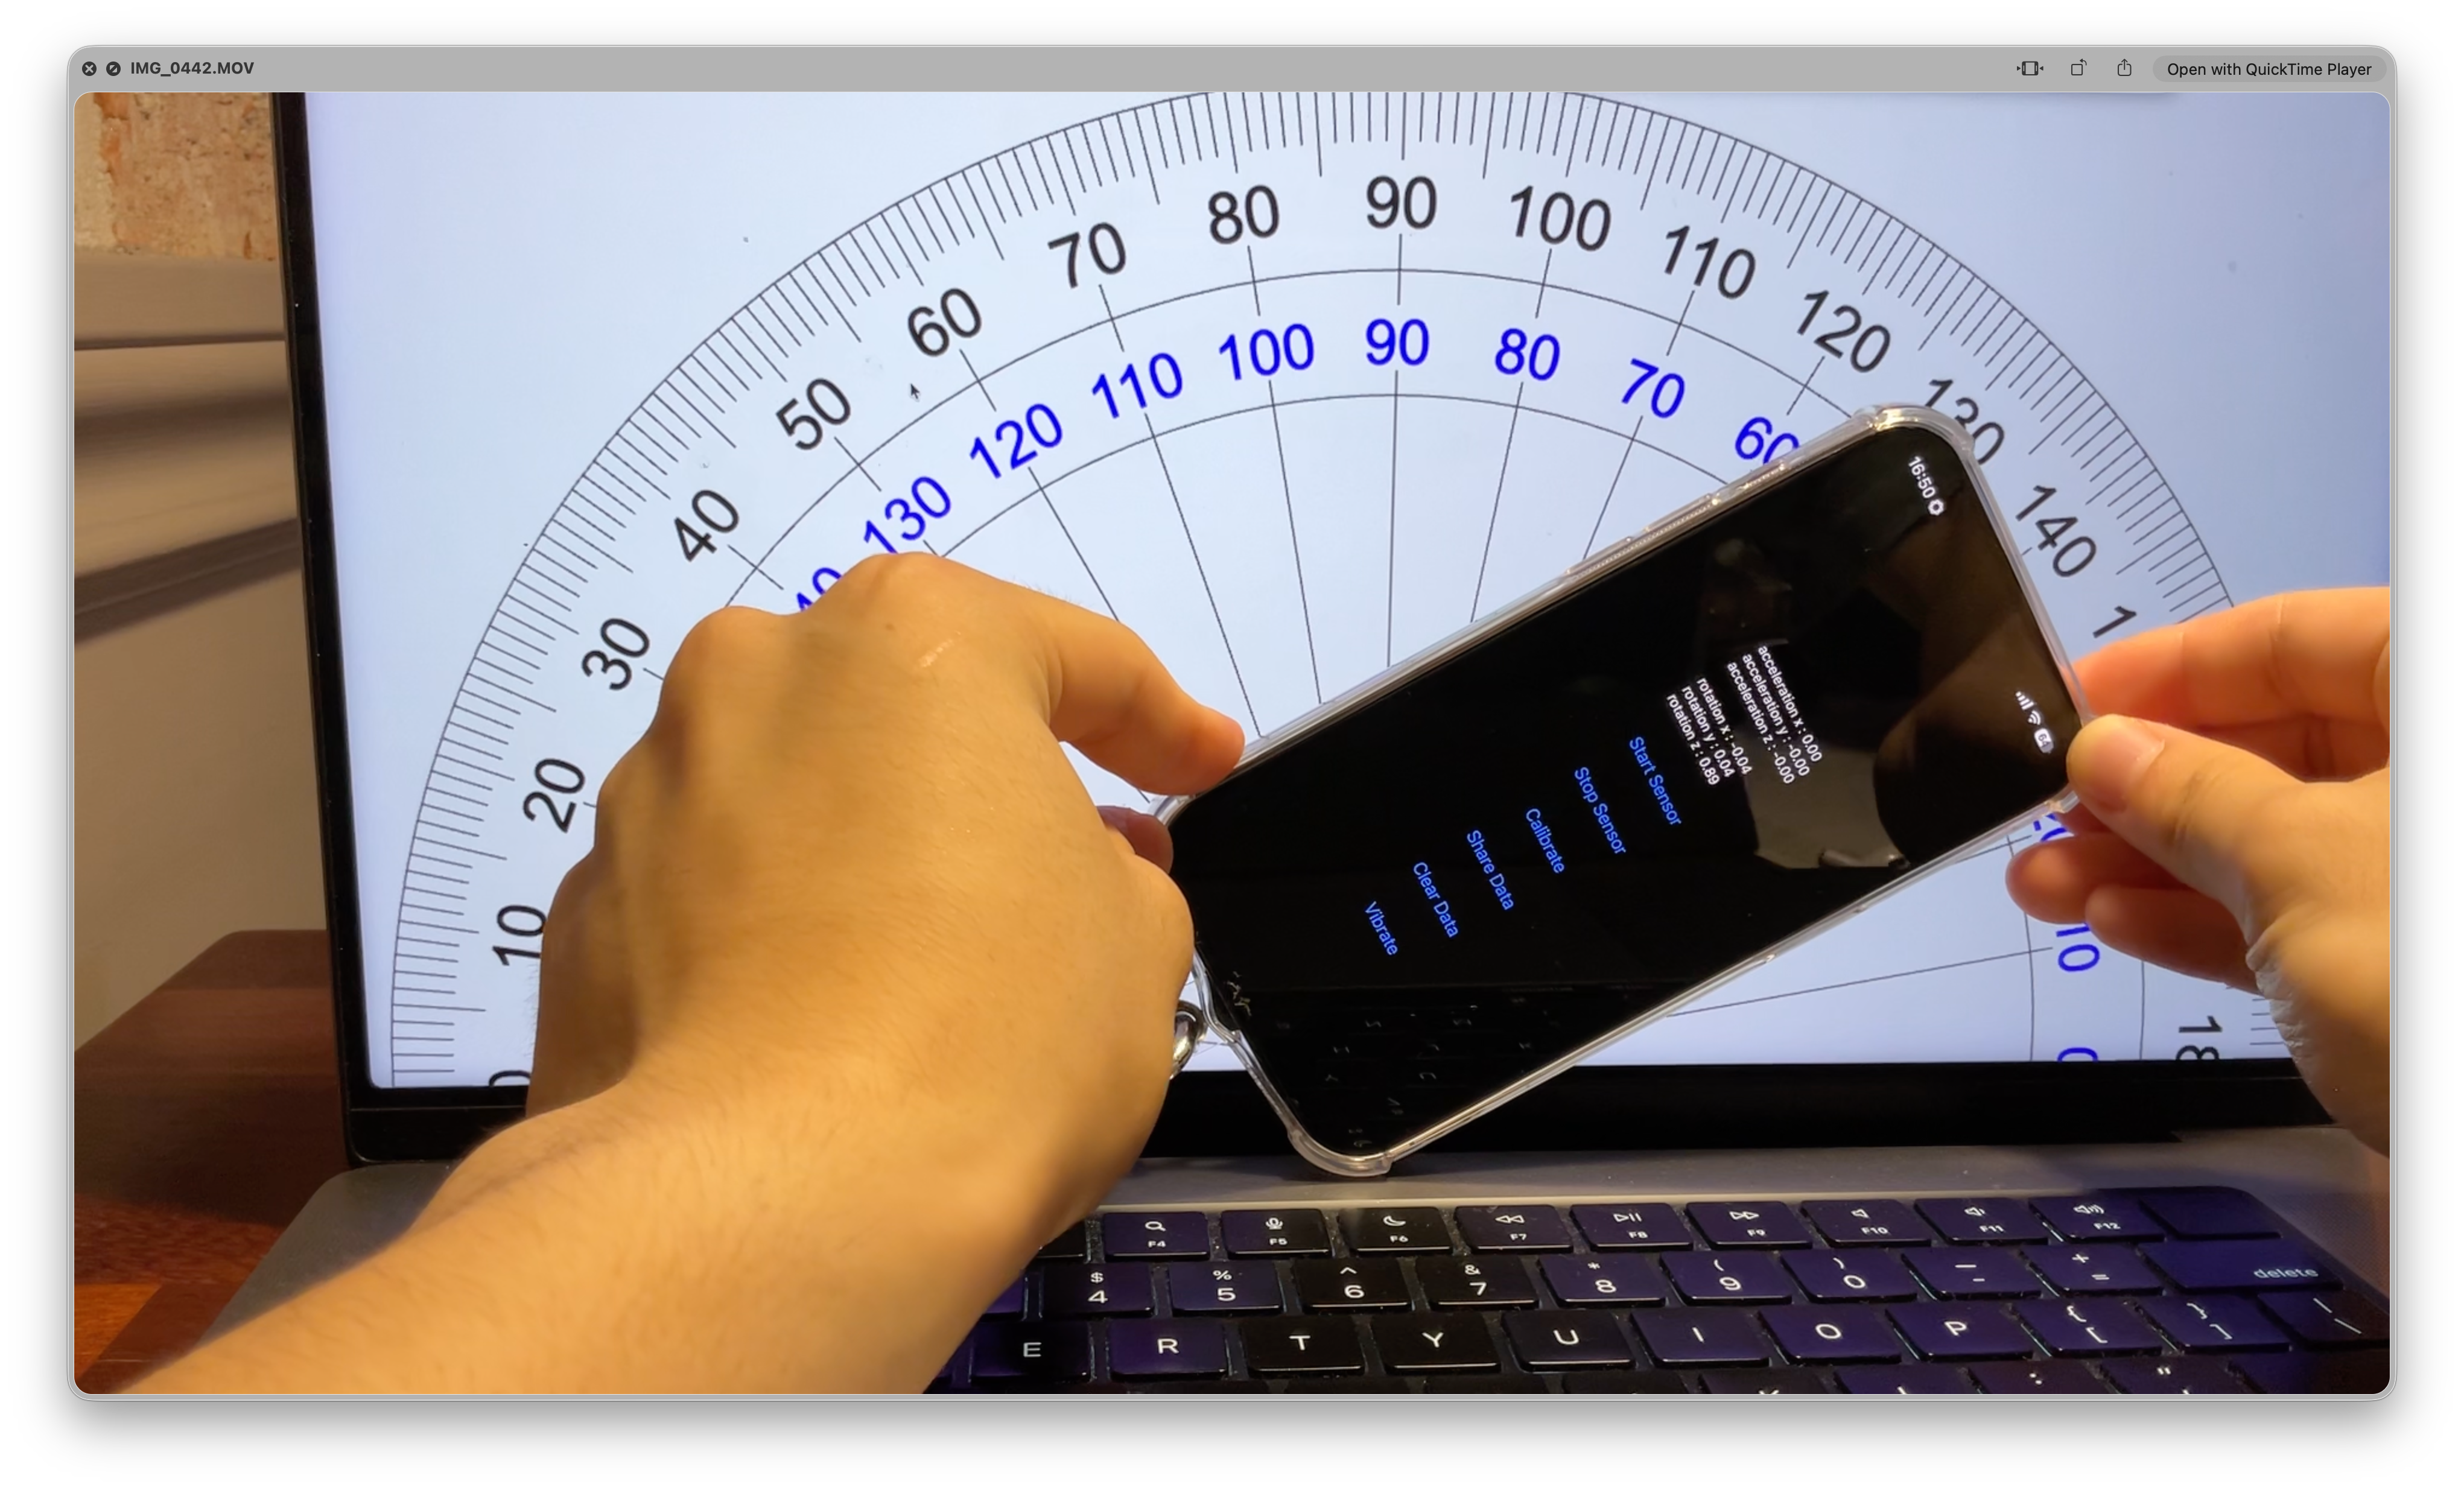
\includegraphics[width=\textwidth]{Images/2_1_3_1.jpg}
        \caption{An image of appropriately estimated orientation}
        \label{fig:2_1_3_1}
    \end{subfigure}
    \begin{subfigure}{0.5\textwidth}
        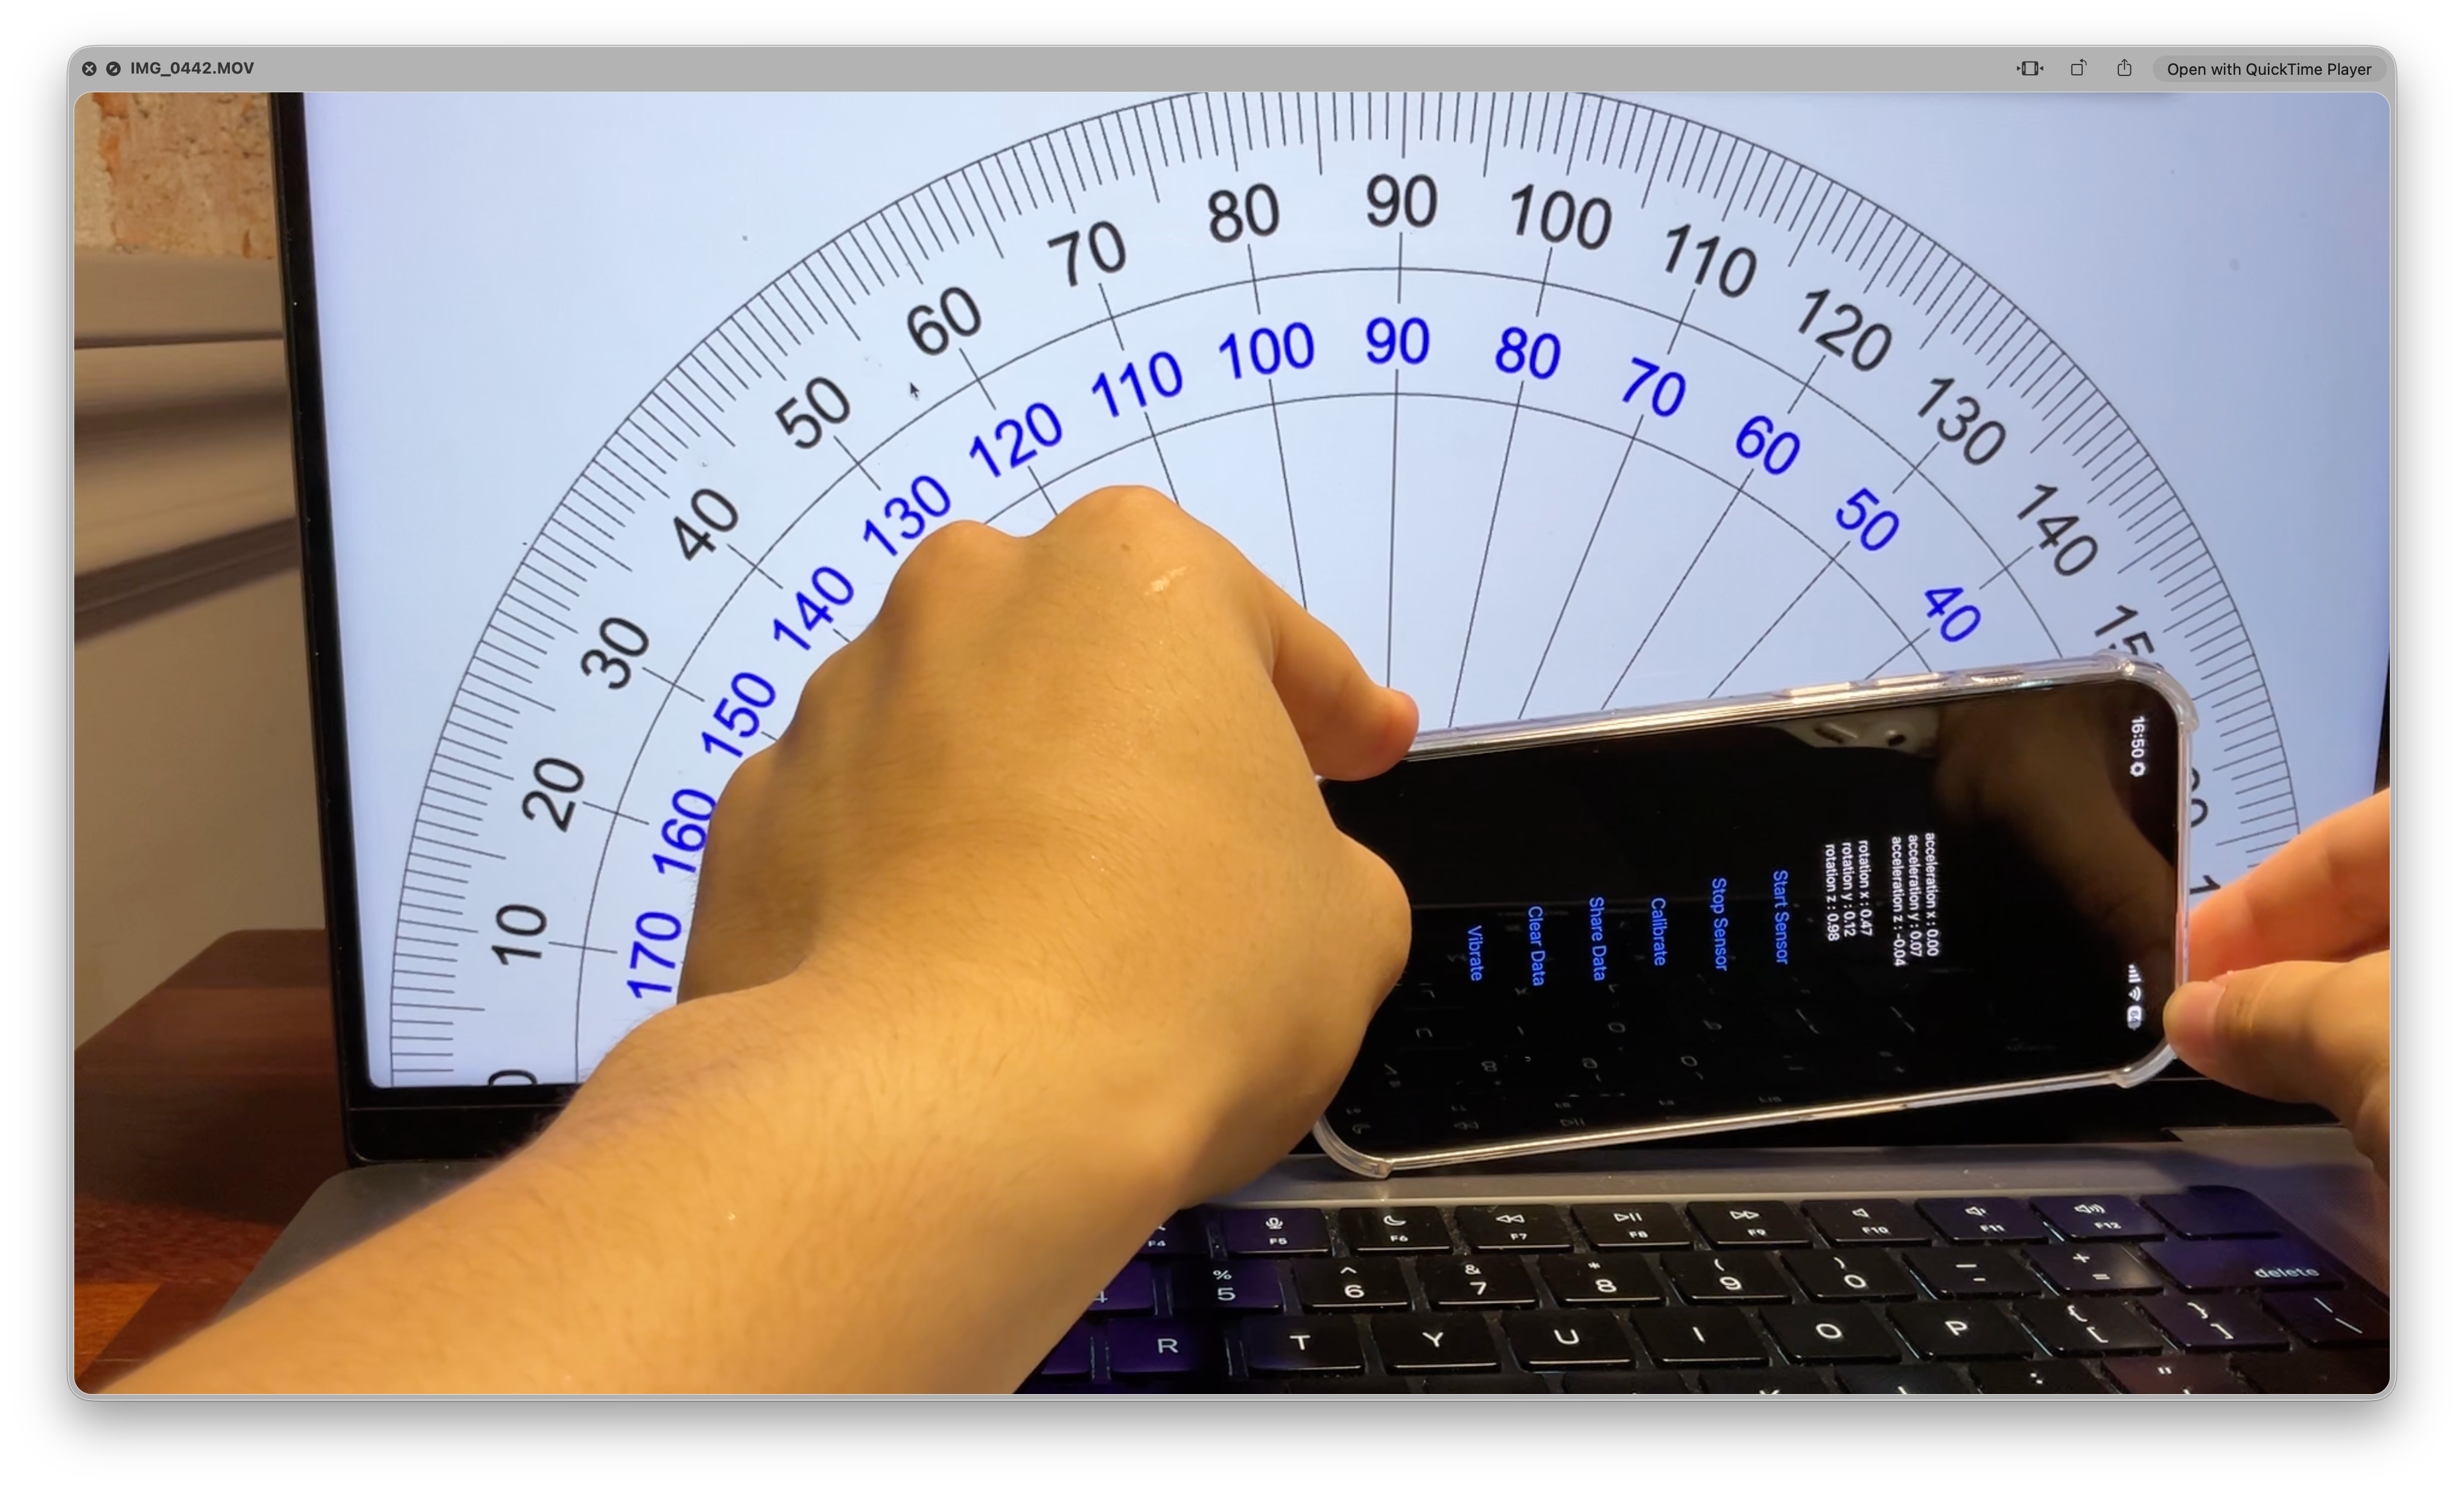
\includegraphics[width=\textwidth]{Images/2_1_3_2.jpg}
        \caption{Inapposite $\theta_x$ caused by $y$, $z$ getting small}
        \label{fig:2_1_3_2}
    \end{subfigure}
    \begin{subfigure}{0.5\textwidth}
        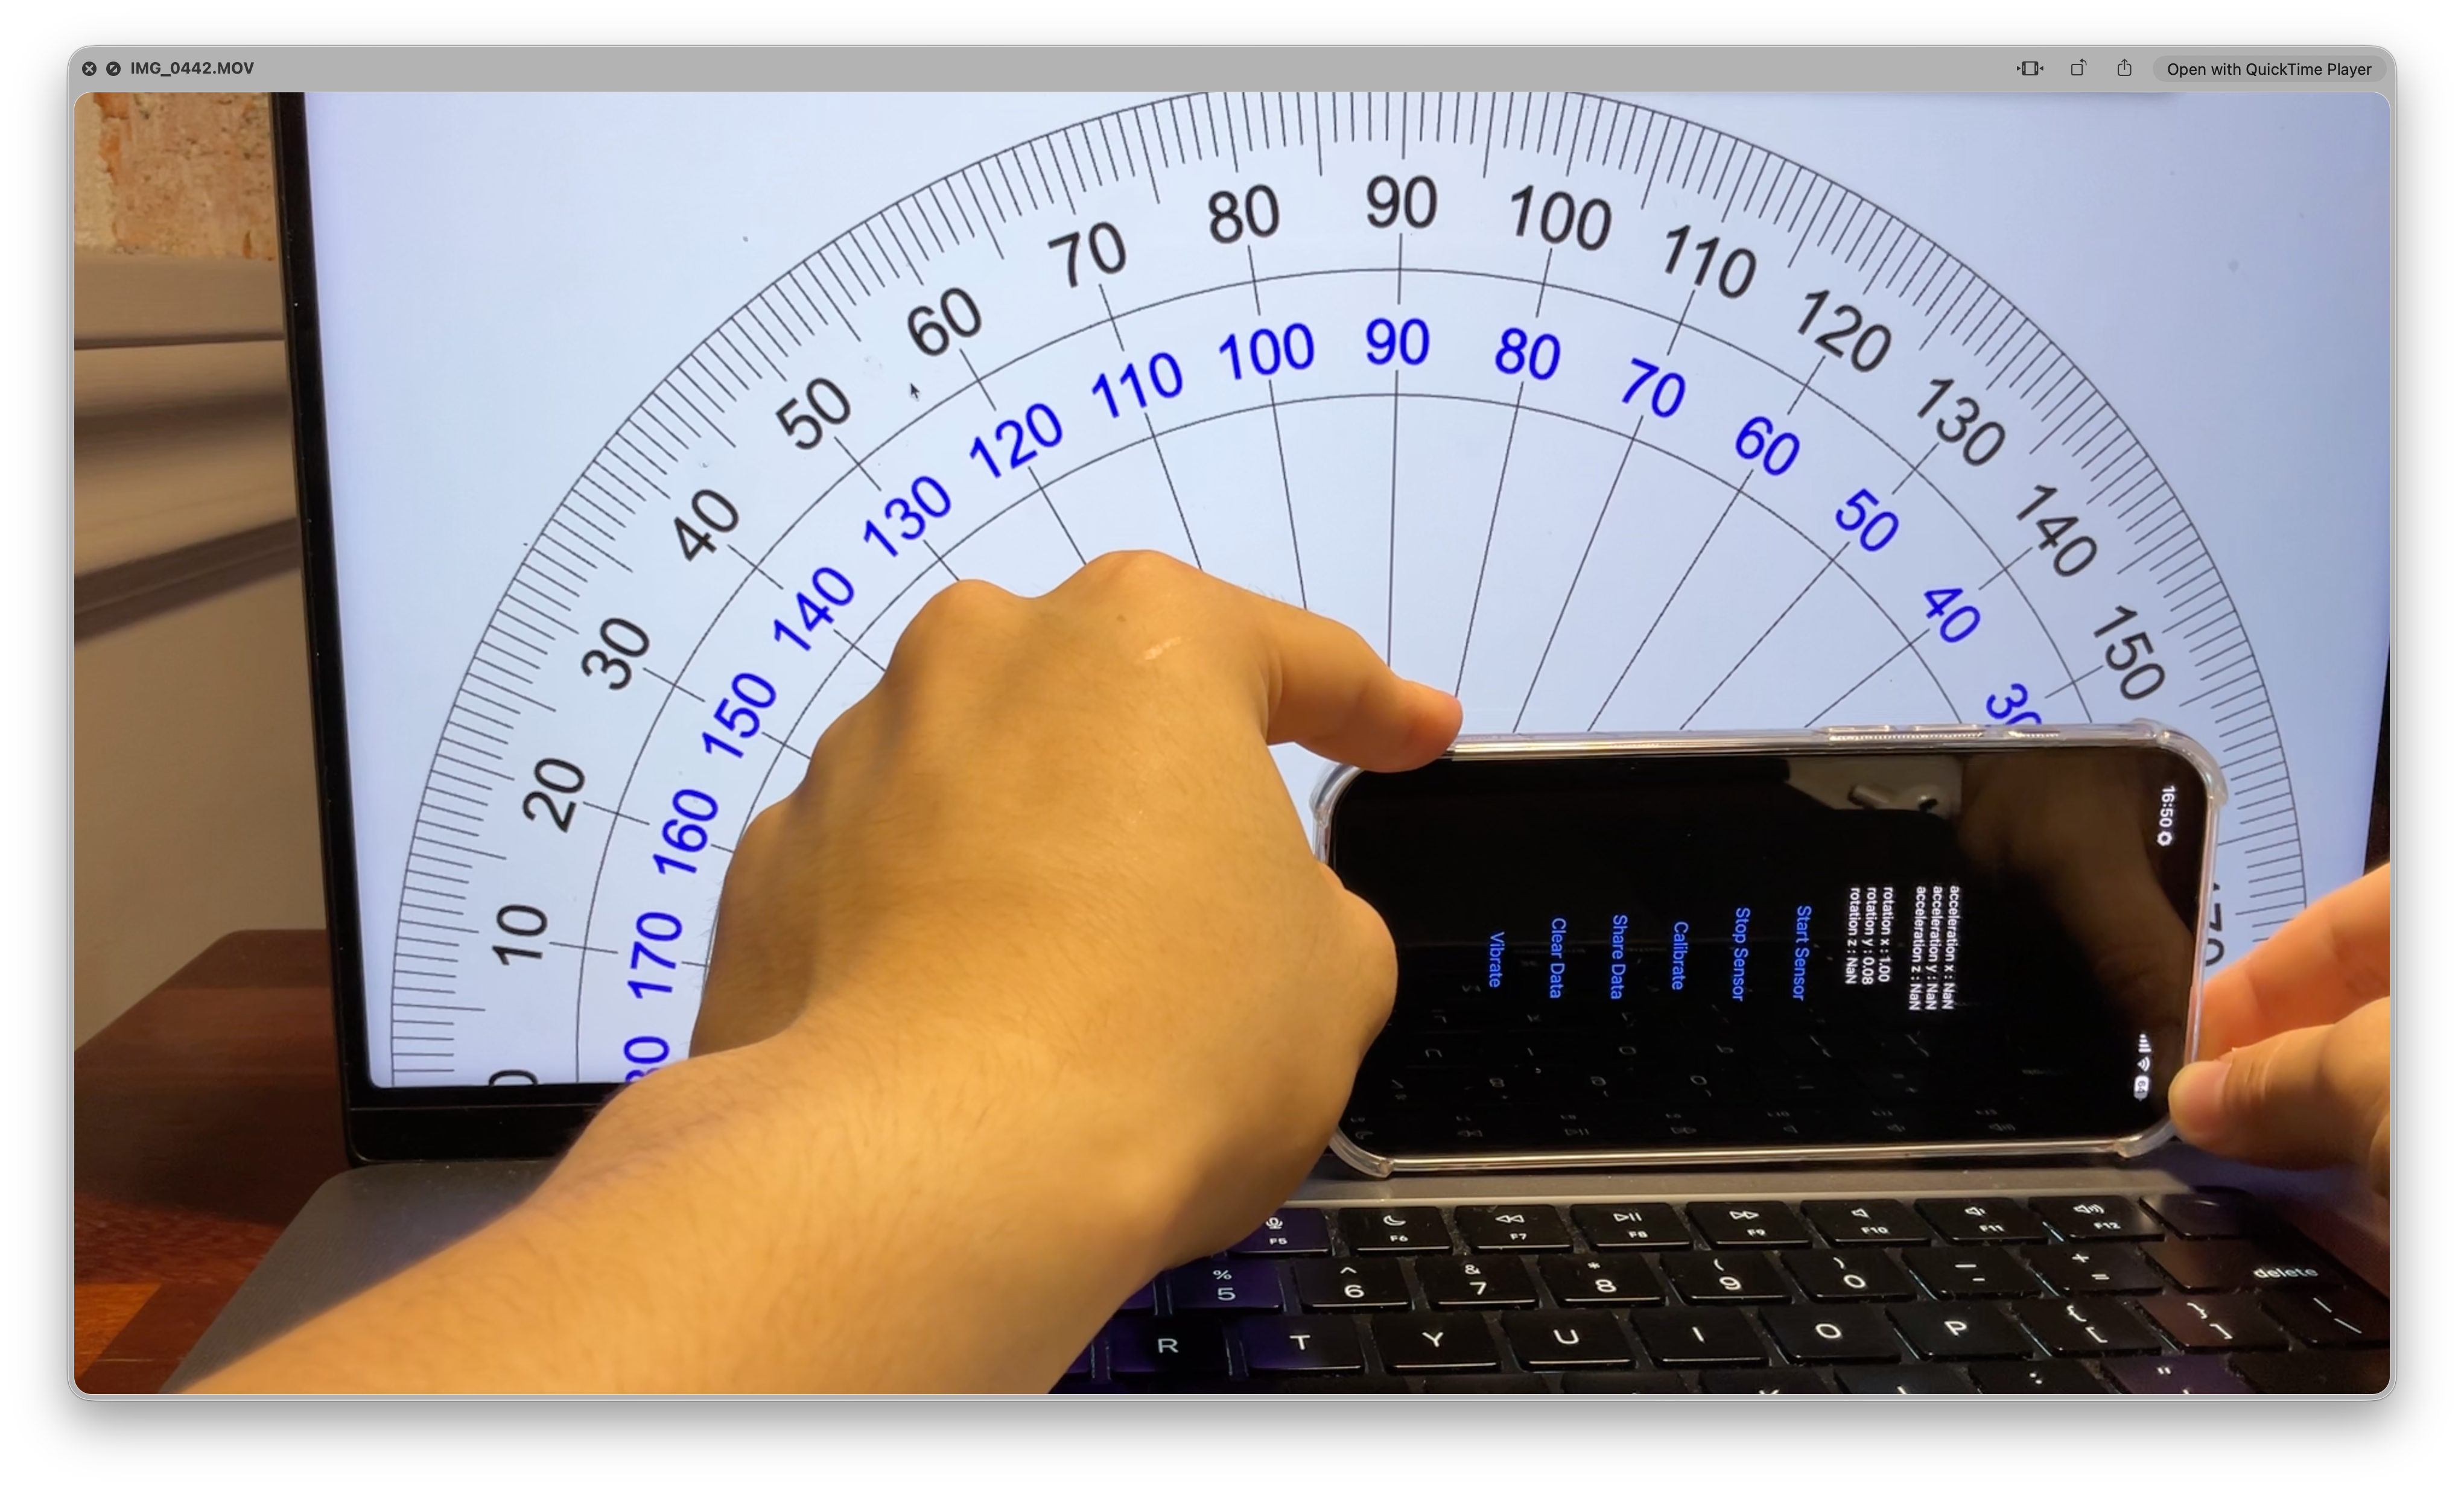
\includegraphics[width=\textwidth]{Images/2_1_3_3.jpg}
        \caption{Error caused by zero $\theta_x$}
        \label{fig:2_1_3_3}
    \end{subfigure}
    \begin{subfigure}{0.5\textwidth}
        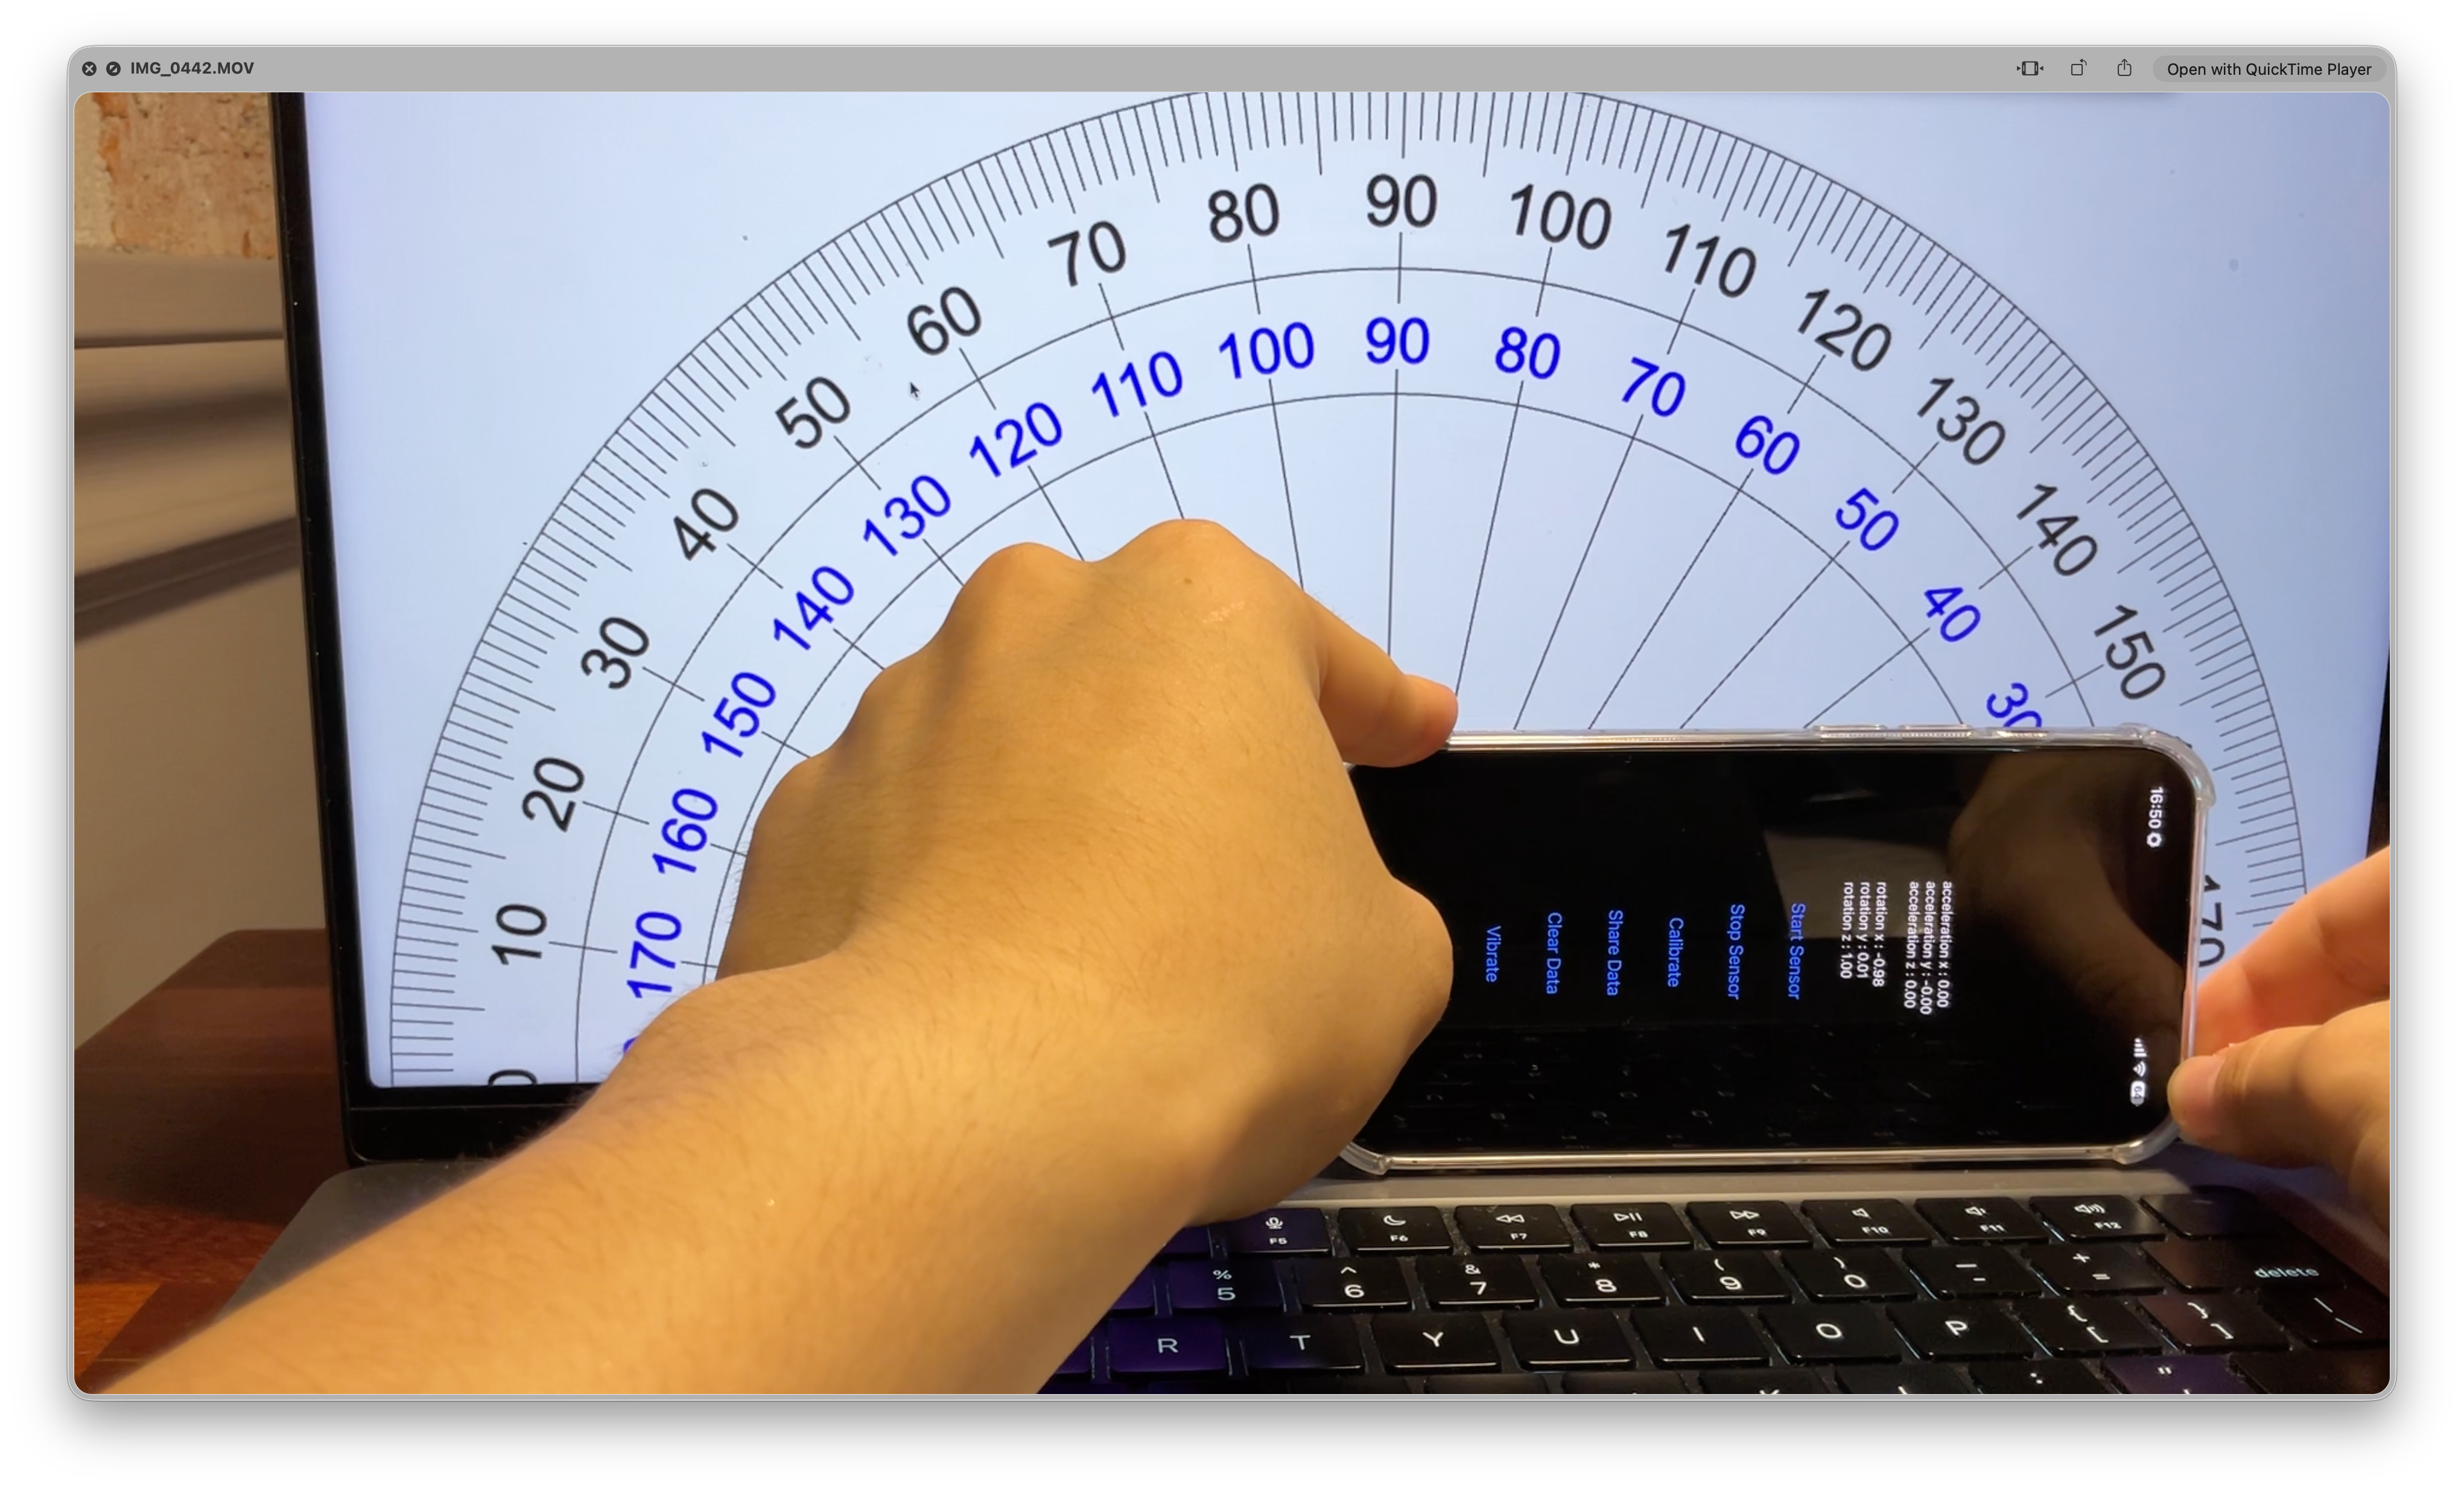
\includegraphics[width=\textwidth]{Images/2_1_3_4.jpg}
        \caption{Inapposite $\theta_x$ caused by $y$ to zero}
        \label{fig:2_1_3_4}
    \end{subfigure}
    \caption{A set of images to find the limit of appropriate estimation of orientation}
    \label{fig:valid_range_test}
\end{figure}


\subsubsection{Orientation Tracking Using the Gyroscope}

To continuously track changes in the smartphone’s orientation during movement, we numerically integrated the gyroscope data over time. The trapezoidal rule was employed for numerical integration to accumulate angular velocity into angular displacement.

Let $t$ denote the current time, and $\delta t$ the time step between measurements. The gyroscope readings collected up to time $t$ are represented as:

\[
\left[
\begin{bmatrix}x_0\\y_0\\z_0\end{bmatrix},
\begin{bmatrix}x_{\delta t}\\y_{\delta t}\\z_{\delta t} \end{bmatrix},
\cdots,
\begin{bmatrix}x_{t-\delta t}\\y_{t-\delta t}\\z_{t-\delta t} \end{bmatrix},
\begin{bmatrix}x_t\\y_t\\z_t \end{bmatrix}
\right]
\]

The orientation of the smartphone at each corresponding time step is given by:

\[
\left[
\begin{bmatrix}\psi_0\\\theta_0\\\phi_0\end{bmatrix},
\begin{bmatrix}\psi_{\delta t}\\\theta_{\delta t}\\\phi_{\delta t}\end{bmatrix},
\cdots,
\begin{bmatrix}\psi_{t-\delta t}\\\theta_{t-\delta t}\\\phi_{t-\delta t} \end{bmatrix},
\begin{bmatrix}\psi_t\\\theta_t\\\phi_t \end{bmatrix}
\right]
\]

Here, the initial gyroscope reading $\begin{bmatrix}x_0&y_0&z_0\end{bmatrix}^\top$ is assumed to be zero, and the initial orientation $\begin{bmatrix}\psi_0&\theta_0&\phi_0\end{bmatrix}^\top$ is taken from the accelerometer-based estimation described in Section~2.1.2.

To compute the current orientation $\begin{bmatrix}\psi_t&\theta_t&\phi_t\end{bmatrix}^\top$, we use the trapezoidal integration method:

\[
\psi_t = \frac{1}{2}(x_t + x_{t - \delta t}) \cdot \delta t + \psi_{t - \delta t}
\]
\[
\theta_t = \frac{1}{2}(y_t + y_{t - \delta t}) \cdot \delta t + \theta_{t - \delta t}
\]
\[
\phi_t = \frac{1}{2}(z_t + z_{t - \delta t}) \cdot \delta t + \phi_{t - \delta t}
\]

Through this integration, the angular velocity data from the gyroscope can be accumulated to track the smartphone’s orientation over time.

\FloatBarrier
\begin{figure}[h]
    \centering
    \includegraphics[width=\textwidth]{2_1_4_1.png}
    \caption{Orientation tracking using trapezoidal integration of gyroscope data}
    \label{fig:gyro_integration}
\end{figure}

\FloatBarrier
\subsubsection{Removal of the Gravity Component}

The smartphone's accelerometer inherently includes the effect of gravity. To isolate the linear acceleration resulting purely from the device’s movement, the gravitational component must be removed. This is accomplished by reconstructing the gravity vector using the orientation estimated in the previous steps.

This process is essentially the inverse of the approach described in Section~2.1.2. When the device is held vertically with its screen facing the user, the expected acceleration due to gravity is:

\[
\begin{bmatrix}
0 \\
-1 \\
0
\end{bmatrix}
\]

By rotating this reference vector according to the current orientation of the device, we can recover the instantaneous gravity vector in the device's coordinate frame.

Let the current orientation of the device be represented by the Euler angles:

\[
\begin{bmatrix}
\psi_t \\
\theta_t \\
\phi_t
\end{bmatrix}
\]

and let the reconstructed gravity vector at time $t$ be denoted as $\vec{g}_t = \begin{bmatrix} g_{x,t} \\ g_{y,t} \\ g_{z,t} \end{bmatrix}$. Then, the gravity vector is given by:

\[
\vec{g}_t =
\begin{bmatrix}
\sin\phi_t \\
-\cos\psi_t \cos\phi_t \\
\sin\psi_t \cos\phi_t
\end{bmatrix}
\]

Finally, the linear acceleration $\vec{A}_t$ caused by the actual movement of the device can be extracted by subtracting the gravity vector from the raw accelerometer reading $\vec{a}_t$:

\[
\vec{A}_t = \vec{a}_t - \vec{g}_t
\]

This process enables accurate detection of motion-induced acceleration ignoring the gravitational effect in real time.

\FloatBarrier
\begin{figure}[h]
    \centering
    \includegraphics[width=\textwidth]{2_1_5_1.png}
    \caption{Estimated gravity component arranged by time}
    \label{fig:gravity_component}
\end{figure}
\FloatBarrier
\begin{figure}[h]
    \centering
    \includegraphics[width=\textwidth]{2_1_5_2.png}
    \caption{Comparing between raw data and gravity component removed data}
    \label{fig:removal_of_gravity_component}
\end{figure}

\FloatBarrier
\subsubsection{Auto Calibration of Orientation}
Since gyroscopes accumulate error over time, the orientation should be periodically recalibrated.
To achieve this, if the magnitude of the acceleration vector is below a certain threshold and the device is able to calibrate its orientation(Section~2.1.3), the orientation is recalibrated through the accelerometer data(Section~2.1.2).


\FloatBarrier
\subsubsection{Noise Removal}
When estimating position from accelerometer data, numerical integration over time often leads to the accumulation of error, resulting in a gradual degradation of accuracy. Figure~\ref{fig:integration_drift} illustrates this phenomenon.

In this experiment, the smartphone was placed flat with its $z$-axis perpendicular to the ground. A simple up-and-down motion was performed by slowly lifting and lowering the device. Theoretically, this movement should result in a sinusoidal pattern in the $z$-axis acceleration, ideally resembling a function of the form $\sin x,\ x \in [0,\ 2\pi]$.

However, the actual measurements deviated significantly from this expected pattern. As shown in the graph, the $z$-axis acceleration (blue line) did not follow the anticipated sine wave. Surprisingly, the $x$-axis—unrelated to the vertical motion—displayed unexpected fluctuations, and the $y$-axis exhibited a divergence trend over time.

These anomalies highlight the impact of sensor noise and the sensitivity of numerical integration to even minor inaccuracies. Small errors in acceleration accumulate rapidly during integration, leading to significant drift in the estimated position that does not correspond to the actual motion.

Therefore, to achieve reliable position tracking, the incorporation of advanced noise reduction techniques is essential.

\FloatBarrier
\begin{figure}[h]
    \centering
    \includegraphics[width=\textwidth]{2_1_6_1.png}
    \caption{Aceleration, speed, position data before noise removal}
    \label{fig:integration_drift}
\end{figure}


\FloatBarrier
\subsubsection{Noise Removal - Using Threshold}

To reduce noise in the accelerometer data, a simple threshold-based filtering technique was initially employed. This method assumes that if the difference between the current and previous sensor readings is below a predefined threshold, the change is not significant and thus the previous value is retained instead of updating with the new measurement.

To determine an appropriate threshold, we analyzed the distribution of accelerometer values when the smartphone was stationary, as shown in Figure~\ref{fig:accel_histogram}. In this state, the $x$ and $y$ axes—which are not affected by gravity—should ideally report values close to zero. However, histogram analysis revealed that values commonly fell within the ranges of $0.14$ to $0.15$ and $-0.16$ to $-0.15$, indicating the presence of noise rather than actual motion. Based on this observation, a threshold of $0.16$ was selected. If the change in acceleration between consecutive time steps was less than this threshold, the previous value was maintained.

Despite its simplicity, this method showed limitations in practice. Experimental results indicated that the filter failed to capture small but meaningful movements and led to accumulated error over time. In other words, the threshold-based approach lacked the sensitivity and precision required for accurate motion tracking in this study.

Consequently, we concluded that a more sophisticated filtering technique is necessary. We plan to implement the Kalman Filter, a widely used and robust method for dynamic state estimation, to improve noise reduction while maintaining responsiveness to actual motion.

\FloatBarrier
\begin{figure}[h]
    \centering
    \includegraphics[width=\textwidth]{2_1_7_1.png}
    \caption{Distribution of accelerometer values when the smartphone is stationary(each graph shows $x$, $y$, and $z$ axis in order)}
    \label{fig:accel_histogram}
\end{figure}

\FloatBarrier
\subsubsection{Noise Removal - Using Kalman Filter}
To overcome the limitations of the simple threshold-based noise removal method discussed earlier, this study applied a more sophisticated filtering technique—the Kalman Filter. The Kalman Filter is widely recognized for its effectiveness in noise suppression and state estimation in time-series data, and is commonly employed in processing various types of sensor data.

In this experiment, the Kalman Filter was applied to the accelerometer measurements to attenuate sensor noise and achieve more stable position estimation. As expected, the filtered output exhibited smoother and more stable transitions compared to the previous method, indicating improved noise reduction performance.

However, in terms of positional accuracy, the Kalman Filter did not yield a significantly meaningful improvement. While it enhanced the visual smoothness of the signal, it was insufficient to correct the inherent drift and integration errors associated with accelerometer-based position estimation.

Therefore, in the next stage of this study, we plan to apply Fast Fourier Transform (FFT) techniques to analyze and suppress noise in the frequency domain, aiming for further improvement in signal fidelity and positional accuracy.

\FloatBarrier
\begin{figure}[h]
    \centering
    \includegraphics[width=\textwidth]{2_1_8_1.png}
    \caption{Comparision between raw accelerometer data and noise reduced accelerometer data using Kalman Filter}
    \label{fig:accel_kalman}
\end{figure}
\FloatBarrier
\begin{figure}[h]
    \centering
    \includegraphics[width=\textwidth]{2_1_8_2.png}
    \caption{Comparision between raw speed data and noise reduced speed data using Kalman Filter}
    \label{fig:speed_kalman}
\end{figure}
\FloatBarrier
\begin{figure}[h]
    \centering
    \includegraphics[width=\textwidth]{2_1_8_3.png}
    \caption{Comparision between raw position data and noise reduced position data using Kalman Filter}
    \label{fig:position_kalman}
\end{figure}

\FloatBarrier
\subsubsection{Noise Removal - Using FFT(Fast Fourier Transform)}
Given the lack of significant improvement in position estimation accuracy after applying the Kalman Filter, this study further explored frequency-based noise reduction techniques using the Fast Fourier Transform (FFT). FFT is a powerful method that converts discrete acceleration signals from the time domain into the frequency domain, allowing for the identification and removal of high-frequency components or unwanted noise.

In this experiment, FFT was applied to the time-series accelerometer data to obtain its frequency spectrum. Frequency components with amplitudes below a threshold of 0.1 were considered insignificant and were eliminated. Subsequently, the Inverse FFT (IFFT) was used to reconstruct the denoised signal in the time domain.

Despite the theoretical effectiveness of this approach, the experimental results showed no substantial improvement in position estimation accuracy. The reconstructed signals appeared cleaner, but the overall trajectory estimation remained inaccurate. Thus, the FFT-based filtering approach, like previous methods, did not yield a practically meaningful enhancement in performance.
\FloatBarrier
\begin{figure}[h]
    \centering
    \includegraphics[width=\textwidth]{2_1_9_1.png}
    \caption{Comparision between raw accelerometer data and noise reduced accelerometer data using FFT}
    \label{fig:accel_fft}
\end{figure}
\FloatBarrier
\begin{figure}[h]
    \centering
    \includegraphics[width=\textwidth]{2_1_9_2.png}
    \caption{Comparision between raw speed data and noise reduced speed data using FFT}
    \label{fig:speed_fft}
\end{figure}
\FloatBarrier
\begin{figure}[h]
    \centering
    \includegraphics[width=\textwidth]{2_1_9_3.png}
    \caption{Comparision between raw position data and noise reduced position data using FFT}
    \label{fig:position_fft}
\end{figure}

\FloatBarrier
\subsubsection{Limit of Accelerometer}
Theoretically, integrating acceleration yields velocity, and a second integration provides position. However, in real-world environments, this process suffers from significant cumulative errors due to the inherent noise present in accelerometer measurements. As a result, accurate position estimation using raw sensor data becomes extremely challenging.

To address this issue, several preprocessing techniques were applied, including Kalman filtering, Fast Fourier Transformation (FFT), and its inverse. While these methods aimed to reduce noise and improve signal quality, they provided only marginal improvements in accuracy when considering the limited computational resources available on mobile devices. In practice, the increased algorithmic complexity outweighed the performance gains, making these approaches less suitable for real-time mobile applications.

In response, this study proposes a novel approach: instead of relying on traditional physics-based integration methods, we remove only the gravitational component from the acceleration data and employ a deep learning model to learn and predict the trajectory of the smartphone. By leveraging data-driven learning rather than error-prone numerical integration, this method aims to alleviate the issue of accumulated drift and achieve more practical and reliable position estimation in mobile environments.


\subsection{Planning Punch Predict Model}

\subsubsection{Using Convolutional Neural Network (CNN)}

The accelerometer data, with gravitational components removed, consist of discrete values along the $x$, $y$, and $z$ axes, collected in temporal order. While it is theoretically possible to incorporate orientation (attitude) information, such an approach incurs excessive computational overhead, making it unsuitable for real-time inference on mobile devices.

This study leverages the observation that a typical punch motion is completed within approximately 0.5 seconds. Based on this, we define one input sequence as a series of 10 acceleration vectors collected at 0.05-second intervals, forming an input shape of $10 \times 3$. To capture both the temporal continuity and the inter-axis interactions, a one-dimensional convolutional layer with a filter size of $3 \times 3$ is applied across the input. This layer extracts relevant spatial-temporal features from the acceleration data.

The convolutional output is then flattened and passed through a fully connected layer, producing four output nodes corresponding to the punch categories. A SoftMax activation is applied to the output layer to obtain a probability distribution over the following punch types: straight, hook, upper cut, and body.

To minimize unnecessary inference and reduce resource consumption on mobile devices, a lightweight pre-processing step is introduced. The model is triggered only when the sum of the absolute values of the $x$, $y$, and $z$ axis accelerations exceeds a predefined threshold. Upon activation, the most recent 10 data points are retrieved from a buffer and fed into the model, ensuring real-time performance with minimal energy cost.

\paragraph{CNN Model Architecture}
\begin{itemize}
    \item \textbf{Input:} $3 \times 10$ accelerometer sequence
    \item \textbf{Convolutional Layer:} Filter size = $3 \times 3$, Stride = 1, Output channels = 4 (up to 8 in experiments)
    \item \textbf{Flatten:} Output vector length = 32 (or up to 64)
    \item \textbf{Fully Connected Layer:} 4 output neurons (one for each punch type)
    \item \textbf{SoftMax:} Outputs class probabilities
    \item \textbf{Threshold-based Trigger:} Executes inference only when acceleration magnitude exceeds predefined threshold
\end{itemize}

\paragraph{Estimated Parameter Count}
\begin{itemize}
    \item Convolutional Weights: $3 \times 3 \times 3 \times 4 = 108$
    \item Fully Connected Weights: $32 \times 4 = 128$
    \item Biases: 4
    \item \textbf{Total:} $\approx 168$ parameters
\end{itemize}


\subsubsection{Using Recurrent Neural Networks (RNN): LSTM and GRU}

While the previous model employed Convolutional Neural Networks (CNN) to process time-sequenced input data, the computational cost per timestep posed limitations for real-time execution and continuous operation on mobile devices.

To address this issue, the current study explores the use of Recurrent Neural Network (RNN) architectures—specifically Long Short-Term Memory (LSTM) and Gated Recurrent Unit (GRU). These models sequentially incorporate information from previous inputs, making them particularly suitable for learning temporal dependencies in time-series data. While CNNs can partially capture time-dependent features, RNNs are inherently designed for temporal modeling and often require fewer parameters, leading to improved efficiency for mobile deployment.

In this model, we also considered the inclusion of temporal phase information alongside the raw accelerometer inputs. Temporal phase, often expressed as a sine value, was incorporated to help the network differentiate between subtle phase shifts in motion. This approach is especially beneficial for recognizing repetitive or periodic movements, and can contribute to enhanced inference precision.

\paragraph{Parameter Comparison of Architectures}

\begin{table}[h]
\centering
\begin{tabular}{|l|c|}
\hline
\textbf{Model Configuration} & \textbf{Estimated Parameter Count} \\
\hline
Conv2D (4 filters) + LSTM (32 units) & $\sim$6,000+ \\
Conv2D (2 filters) + GRU (8 units) & $\sim$800--1,000 \\
\hline
\end{tabular}
\caption{Comparison of CNN-RNN hybrid models in terms of parameter count}
\end{table}

Although LSTM offers a higher capacity for modeling complex temporal patterns, it also introduces substantial computational overhead. This overhead can be problematic in mobile environments where real-time inference is required. In contrast, GRU provides a more lightweight alternative, reducing the parameter count by more than 85\% while maintaining competitive performance.

Given the trade-offs between accuracy and computational cost, GRU was found to be a more practical choice for real-time, resource-constrained applications such as smartphone-based punch classification.

\subsubsection{Using Hybrid Architecture: CNN + RNN}

To effectively process the sequential accelerometer data, this study adopts a hybrid architecture combining a Convolutional Neural Network (CNN) and a Recurrent Neural Network (RNN). In this configuration, the CNN is responsible for extracting local spatial features at each time step, while the RNN captures the temporal dependencies across the entire sequence.

The model operates as follows:

\begin{quote}
\begin{center}
Time $t_1$: Input $(3 \times 3)$ → CNN → Feature Vector $\mathbf{v}_1$ \\
Time $t_2$: Input $(3 \times 3)$ → CNN → Feature Vector $\mathbf{v}_2$ \\
\quad$\vdots$ \\
Time $t_t$: Input $(3 \times 3)$ → CNN → Feature Vector $\mathbf{v}_t$ \\[1ex]

RNN([\,$\mathbf{v}_1$, $\mathbf{v}_2$, ..., $\mathbf{v}_t$\,]) → Output Class (0--3)
\end{center}
\end{quote}

In other words, for each time step, a $3 \times 3$ acceleration matrix is passed through a CNN to extract a compressed feature vector. These feature vectors, representing the motion characteristics over time, are then sequentially input into an LSTM (or GRU) layer to predict the final class label.

This architecture effectively combines the strengths of both networks: CNNs efficiently learn spatial representations from short-term input windows, while RNNs capture longer-term temporal dynamics, making the model well-suited for fine-grained motion classification such as punch detection.







\subsection{Preparing Punch Dataset}

\subsubsection{Data Construction}

To develop an effective deep learning-based punch recognition model, we constructed time-series input data derived from smartphone sensor readings and created corresponding labeled datasets.

The raw sensor data were collected using the built-in Inertial Measurement Unit (IMU), which includes a 3-axis accelerometer, 3-axis gyroscope, and 3-axis magnetometer. However, the magnetometer data were excluded from the model due to high noise levels and their limited contribution to motion recognition. Similarly, gyroscope data—although useful for orientation estimation—were also excluded from the input features to reduce model complexity. If computational resources permit, orientation data derived from gyroscope integration may be incorporated in future versions.

Based on this setup, the input features $\mathbf{X}$ consist of stacked 3-axis accelerometer readings over a fixed time window $T$. Each sample is a 3-dimensional tensor of shape $(T, 3, 3)$, where each element corresponds to a $3 \times 3$ matrix containing three consecutive accelerometer readings (for temporal locality) across the $x$, $y$, and $z$ axes.

The target label $\mathbf{y}$ corresponds to the punch class annotated at each timestamp. The class labels are defined as follows:  
\texttt{0}: No punch detected,  
\texttt{1}: Straight,  
\texttt{2}: Hook,  
\texttt{3}: Uppercut,  
\texttt{4}: Body punch.

For training, class labels are initially provided as strings (e.g., `"Straight"`, `"None"`, etc.), and then encoded either as one-hot vectors for use with the \texttt{categorical\_crossentropy} loss function, or as integer indices for \texttt{sparse\_categorical\_crossentropy}, depending on the model's configuration.

\begin{lstlisting}[language=Python, caption={Example input-output data format}]
# Example shape: (T, 3, 3)
X = [
  [[...], [...], [...]],  # t1: 3-axis x 3 time steps
  [[...], [...], [...]],  # t2
  ...
  [[...], [...], [...]],  # tT
]

y = [
  "None",
  "Straight",
  "None",
  ...
  "None",
]
\end{lstlisting}

This labeling scheme ensures that the model learns not only to recognize punch gestures, but also to distinguish them from idle or transitional motion patterns. The model is trained to output a class prediction at each time step, enabling real-time recognition of punch events as they occur.



\subsubsection{Data Augmentation Using Sliding Window}

To increase the size of the training dataset and improve model generalizability, we adopted a **sliding window algorithm** to generate overlapping time-series samples. This method is particularly effective for time-dependent sensor data, as it allows the model to learn from slightly shifted but semantically similar motion sequences.

Given a raw data stream $\mathbf{D} = [\mathbf{d}_1, \mathbf{d}_2, ..., \mathbf{d}_n]$, where each $\mathbf{d}_i$ is a $3 \times 3$ matrix representing three consecutive accelerometer readings across the $x$, $y$, and $z$ axes, we construct input sequences $\mathbf{X}$ of fixed length $T$ using a sliding window of size $T$ and stride $1$. The label $\mathbf{y}$ for each sequence is assigned based on the punch class at the last timestep of the window.

The following Python snippet illustrates the implementation of this process:

\begin{lstlisting}[language=Python, caption={Sliding window algorithm for data augmentation}]
WINDOW = 20  # sequence length T

X_list = []
y_list = []

for i in range(len(data) - WINDOW):
    window = data[i:i+WINDOW]  # shape: (WINDOW, 3, 3)
    label = label_list[i + WINDOW - 1]  # label at the last timestep
    X_list.append(window)
    y_list.append(label)
\end{lstlisting}

This approach enables a significant increase in the number of training samples, while preserving the temporal structure of the original data. Additionally, by assigning the label based on the final frame in each window, the model is encouraged to predict punch classes based on their full temporal context, rather than instantaneous changes.






\subsubsection{Data Accumulation}
To accumulate the punch dataset, we collected data from multiple users performing various punch types. Each user was instructed to perform a series of punches while holding the smartphone in a same grip, as shown in Figure~\ref{fig:phone_grips}.

The gravity component of the accelerometer is removed each time interval.

\FloatBarrier
\begin{figure}[h]
    \centering
    \begin{subfigure}{0.33\textwidth}
        \centering
        \includegraphics[width=\textwidth]{2_3_3_1.png}
        \label{fig:grip_1}
    \end{subfigure}%
    \begin{subfigure}{0.33\textwidth}
        \centering
        \includegraphics[width=\textwidth]{2_3_3_2.png}
        \label{fig:grip_2}
    \end{subfigure}%
    \begin{subfigure}{0.33\textwidth}
        \centering
        \includegraphics[width=\textwidth]{2_3_3_3.png}
        \label{fig:grip_3}
    \end{subfigure}
    \caption{A set of images showing the smartphone being held (refer to Figure~\ref{fig:accelerometer} for orientation, the dotted lines are negative axes)}
    \label{fig:phone_grips}
\end{figure}

\FloatBarrier
\subsection{Analyzing Punch Data}

\FloatBarrier
\begin{figure}[h]
    \centering
    \includegraphics[width=\textwidth]{straight_user_input.png}
    \caption{Punch data collected from a user performing a straight punch, red dots indicate the peak of the punch}
    \label{fig:straight_user_input}
\end{figure}

\FloatBarrier
\begin{figure}[h]
    \centering
    \includegraphics[width=\textwidth]{punch_data.png}
    \caption{Punch data collected from a user performing various punches(straight, body, hook, uppercut), each colored dot indicates the punch}
    \label{fig:punch_data}
\end{figure}








\subsection{Building Punch Predict Model}









\FloatBarrier
\subsection{Evaluating Various Punch Predict Model}











\subsection{Developing Smartphone Application}

\subsubsection{UI/UX}



\section{Results}

\end{document}
